% Use only LaTeX2e, calling the article.cls class and 12-point type.
\documentclass[12pt]{article}

% Users of the {thebibliography} environment or BibTeX should use the
% scicite.sty package, downloadable from *Science* at
% www.sciencemag.org/about/authors/prep/TeX_help/ .
% This package should properly format in-text
% reference calls and reference-list numbers.

% Science template required packages
\usepackage{scicite}

\usepackage{times}

% add-ons for rticles
% based on arxiv.sty
\usepackage[utf8]{inputenc} % allow utf-8 input
\usepackage[T1]{fontenc}    % use 8-bit T1 fonts
\usepackage[hidelinks]{hyperref}       % hyperlinks
\usepackage{url}            % simple URL typesetting
\usepackage{booktabs}       % professional-quality tables
\usepackage{amsfonts}       % blackboard math symbols
\usepackage{nicefrac}       % compact symbols for 1/2, etc.
\usepackage{microtype}      % microtypography
\usepackage{lipsum}
\usepackage{graphicx}

% the basics
\usepackage{amsmath}
\usepackage{calc}
\usepackage{tabularx}

% for figure adjustment
\usepackage{placeins}
\usepackage{flafter}




% tightlist command for lists without linebreak
\providecommand{\tightlist}{%
  \setlength{\itemsep}{0pt}\setlength{\parskip}{0pt}}

% From pandoc table feature
\usepackage{longtable,booktabs,array}
\usepackage{calc} % for calculating minipage widths
% Correct order of tables after \paragraph or \subparagraph
\usepackage{etoolbox}
\makeatletter
\patchcmd\longtable{\par}{\if@noskipsec\mbox{}\fi\par}{}{}
\makeatother
% Allow footnotes in longtable head/foot
\IfFileExists{footnotehyper.sty}{\usepackage{footnotehyper}}{\usepackage{footnote}}
\makesavenoteenv{longtable}

% Pandoc citation processing
\newlength{\csllabelwidth}
\setlength{\csllabelwidth}{3em}
\newlength{\cslhangindent}
\setlength{\cslhangindent}{1.5em}
% for Pandoc 2.8 to 2.10.1
\newenvironment{cslreferences}%
  {}%
  {\par}
% For Pandoc 2.11+
\newenvironment{CSLReferences}[2] % #1 hanging-ident, #2 entry spacing
 {% don't indent paragraphs
  \setlength{\parindent}{0pt}
  % turn on hanging indent if param 1 is 1
  \ifodd #1 \everypar{\setlength{\hangindent}{\cslhangindent}}\ignorespaces\fi
  % set entry spacing
  \ifnum #2 > 0
  \setlength{\parskip}{#2\baselineskip}
  \fi
 }%
 {}
\usepackage{calc} % for calculating minipage widths
\newcommand{\CSLBlock}[1]{#1\hfill\break}
\newcommand{\CSLLeftMargin}[1]{\parbox[t]{\csllabelwidth}{#1}}
\newcommand{\CSLRightInline}[1]{\parbox[t]{\linewidth - \csllabelwidth}{#1}\break}
\newcommand{\CSLIndent}[1]{\hspace{\cslhangindent}#1}



% The following parameters seem to provide a reasonable page setup.

\topmargin 0.0cm
\oddsidemargin 0.2cm
\textwidth 16cm
\textheight 21cm
\footskip 1.0cm


%The next command sets up an environment for the abstract to your paper.
\usepackage{setspace}

\newenvironment{sciabstract}{%
\begin{quote} \singlespacing}
{\end{quote}}


% If your reference list includes text notes as well as references,
% include the following line; otherwise, comment it out.

\renewcommand\refname{References and Notes}

% The following lines set up an environment for the last note in the
% reference list, which commonly includes acknowledgments of funding,
% help, etc.  It's intended for users of BibTeX or the {thebibliography}
% environment.  Users who are hand-coding their references at the end
% using a list environment such as {enumerate} can simply add another
% item at the end, and it will be numbered automatically.

\newcounter{lastnote}
\newenvironment{scilastnote}{%
\setcounter{lastnote}{\value{enumiv}}%
\addtocounter{lastnote}{+1}%
\begin{list}%
{\arabic{lastnote}.}
{\setlength{\leftmargin}{.22in}}
{\setlength{\labelsep}{.5em}}}
{\end{list}}


% Include your paper's title here

\title{\bf Mainstreaming Race Science}


% Place the author information here.  Please hand-code the contact
% information and notecalls; do *not* use \footnote commands.  Let the
% author contact information appear immediately below the author names
% as shown.  We would also prefer that you don't change the type-size
% settings shown here.


\author{
Daniel J. Hicks,\textsuperscript{1}\textsuperscript{*}
and Emilio Lobato\textsuperscript{1}
\\
\\
\normalsize{\textsuperscript{1}University of California, Merced}\\
\\
\textsuperscript{*}Corresponding author: Daniel J. Hicks, \href{mailto:dhicks4@ucmerced.edu}{\nolinkurl{dhicks4@ucmerced.edu}}.
}

% Include the date command, but leave its argument blank.

\date{}



%%%%%%%%%%%%%%%%% END OF PREAMBLE %%%%%%%%%%%%%%%%



\begin{document}
% Double-space the manuscript.

\baselineskip24pt

% Make the title.

\maketitle

% Place your abstract within the special {sciabstract} environment.

\begin{sciabstract}
\emph{{[}structured{]}}
\end{sciabstract}

\hypertarget{introduction}{%
\section*{Introduction}\label{introduction}}

\emph{{[}hey you should read this paper{]}}

\emph{{[}incorporate def'ns{]}}

\begin{description}
\tightlist
\item[scientific racism]
purporting to justify racial inequality and colonialism by appealing to the epistemic authority of science
\item[race science]
(pseudo-)scientific research that can be utilized for scientific racism
\item[race science discourse]
treating race science as a legitimate area of scientific research; this includes methodological critiques of race science and empirical tests that falsify race science hypotheses
\end{description}

\begin{itemize}
\tightlist
\item
  pre-20th century history of race concepts and race science
\item
  expansion and contraction of racialized terms over time
\end{itemize}

\hypertarget{race-science-1910-1960}{%
\section*{Race science 1910-1960}\label{race-science-1910-1960}}

\hypertarget{the-rise-and-fall-of-eugenics}{%
\subsection*{The rise and fall of eugenics}\label{the-rise-and-fall-of-eugenics}}

\emph{{[}write this{]}}

\begin{itemize}
\tightlist
\item
  scientific racism is thoroughly entangled with eugenics, but still conceptually distinct (Slobodian 2023)

  \begin{itemize}
  \tightlist
  \item
    sterilization laws focused on categories of criminality and mental ability, rather than race per se
  \item
    contemporary defenders of eugenics at least sometimes claim to oppose racism
  \item
    claims of innate racial differences in intelligence can be made without dysgenic prophecies of a rapidly-expanding biological underclass
  \end{itemize}
\item
  1910: Davenport founds Eugenics Records Office at Cold Spring Harbor
\item
  1926: NRC ``Committee on the Negro'' includes both Davenport and Boas: ``neither was influential enough to veto his rival's participation'' (Barkan 1992, 113)
\item
  1930s: \emph{Coming of Age in Samoa} (Mead 1928) popularizes cultural anthropology, ``free{[}ing{]} anthropology from the shackles of biology'' (Barkan 1992, 134)
\item
  1937: Pioneer Fund is founded to ``support academic research and the '{[}sic{]}dissemination of information, into the `problem of heredity and eugenics' and `the problems of race betterment'\,'' (Mehler 1989, 21, quoting Laughlin)
\item
  1940: Carnegie Institute defunds Eugenics Records Office
\item
  1950: ``For all practical social purposes `race' is not so much a biological phenomenon as a social myth'' (Beaglehole et al. 1950; though see Brattain 2007)
\end{itemize}

\hypertarget{brown-v-board-and-mankind-quarterly}{%
\subsection*{\texorpdfstring{\emph{Brown v Board} and \emph{Mankind Quarterly}}{Brown v Board and Mankind Quarterly}}\label{brown-v-board-and-mankind-quarterly}}

Histories of scientific racism in the second half of the twentieth century have often emphasized the parascholarly journal \emph{Mankind Quarterly} (MQ) \cite{
MehlerFoundationFascismNew1989,
WinstonScienceServiceFar1998,
SchafferScientificRacismAgain2007,
SainiSuperiorReturnRace2019,
WinstonScientificRacismNorth2020,
AdamsMisAppropriationBiological2021,
SainiDraperMillionsPhilanthropic2022
}, with or without its connections to PF. MQ was founded in 1960 by biologist R. Ruggles Gates (1882-1962), psychologist Henry Garrett (1894-1973), and non-academic anthropologist G. Robert Gayre (self-styled as ``Gayre of Gayre and Nigg''; 1907-1996). Gates' professional status was closely tied to eugenics and the explicit scientific racism of the 1920s, and he had been thoroughly marginalized in the wake of World War II \cite{WinstonScienceServiceFar1998}. In contrast, Garrett had been president of the American Psychological Association in 1946 and chair of Psychology at Columbia from 1941 to 1955 \emph{{[}cite{]}}.

In the landmark case \emph{Brown v Board of Education of Topeka} (1954), the US Supreme Court had banned \emph{de jure} educational segregation. The Court's decision relied on expert testimony from psychologists and education researchers; but the segregationists had also put forward their own experts, including Henry Garrett \cite{WinstonScienceServiceFar1998, JacksonScienceSegregationRace2005, SchafferScientificRacismAgain2007}. Shortly after \emph{Brown}, Garrett left Columbia, taking a visiting position at the University of Virginia, and becoming increasingly involved in segregationist, eugenicist, and even the neofascist Northern League.

In the context of \emph{Brown}, MQ was created as what contemporary scholars call an ``echo chamber'' \cite{FernandezPintoKnowBetterNot2017}, a favorable venue for race scientists to publish their views, on the grounds that an ``equalitarian dogma'' created a censorious ``taboo'' against their research in mainstream publications \cite{TuckerFundingScientificRacism2002, JacksonMythicalTabooRace2020}. Historians, philosophers, and sociologists of science have shown that echo chambers have been a key part of the ``tobacco strategy,'' used by numerous regulated industries --- most infamously tobacco, but also fossil fuels and chemical manufacturing, among others --- to ``manufacture doubt'' and delay regulation to protect public and environmental health \emph{{[}cites{]}}.

In light of the origins of MQ, the significant attention paid to the journal by historians of scientific racism, and contemporary research on the ``tobacco strategy,'' it is surprising that MQ did not play a significant role in nurturing race science.

\hypertarget{mankind-quarterly-and-pioneer-funded-researchers}{%
\section*{\texorpdfstring{\emph{Mankind Quarterly} and Pioneer-funded researchers}{Mankind Quarterly and Pioneer-funded researchers}}\label{mankind-quarterly-and-pioneer-funded-researchers}}

We identified 16 researchers who had received funding from Pioneer; 14 of these researchers had profiles in the Web of Science (WoS) author search \emph{{[}table + WoS pub coucnt{]}}, allowing us identify 13 WoS-indexed journals that had published 6 or more of these authors. See Table \ref{tab:researchers}.

\begin{longtable}[]{@{}lrl@{}}
\caption{\label{tab:researchers} Pioneer-funded researchers. Either identified in \emph{{[}cite{]}} or named on Pioneer's website, along with identified discipline and WoS author search result counts.}\tabularnewline
\toprule
\endhead
Thomas J. Bouchard, Jr. & psychology & \\
Brunetto Chiarelli & anthropology & \\
Hans Eysenck & psychology & \\
Robert Gordon & sociology & \\
Linda Gottfredson & psychology & \\
Garrett Hardin & ecology & \\
Joseph M. Horn & psychology & \\
Lloyd Humphreys & psychology & \\
Arthur Jensen & psychology & \\
Michael Levin & philosophy & \\
Richard Lynn & psychology & \\
R. Travis Osborne & psychology & \\
J. Phillippe Rushton & psychology & \\
Audrey M. Shuey & psychology & \\
Philip A. Vernon & psychology & \\
Daniel Vining, Jr. & demography & \\
\bottomrule
\end{longtable}

\begin{figure}
\centering
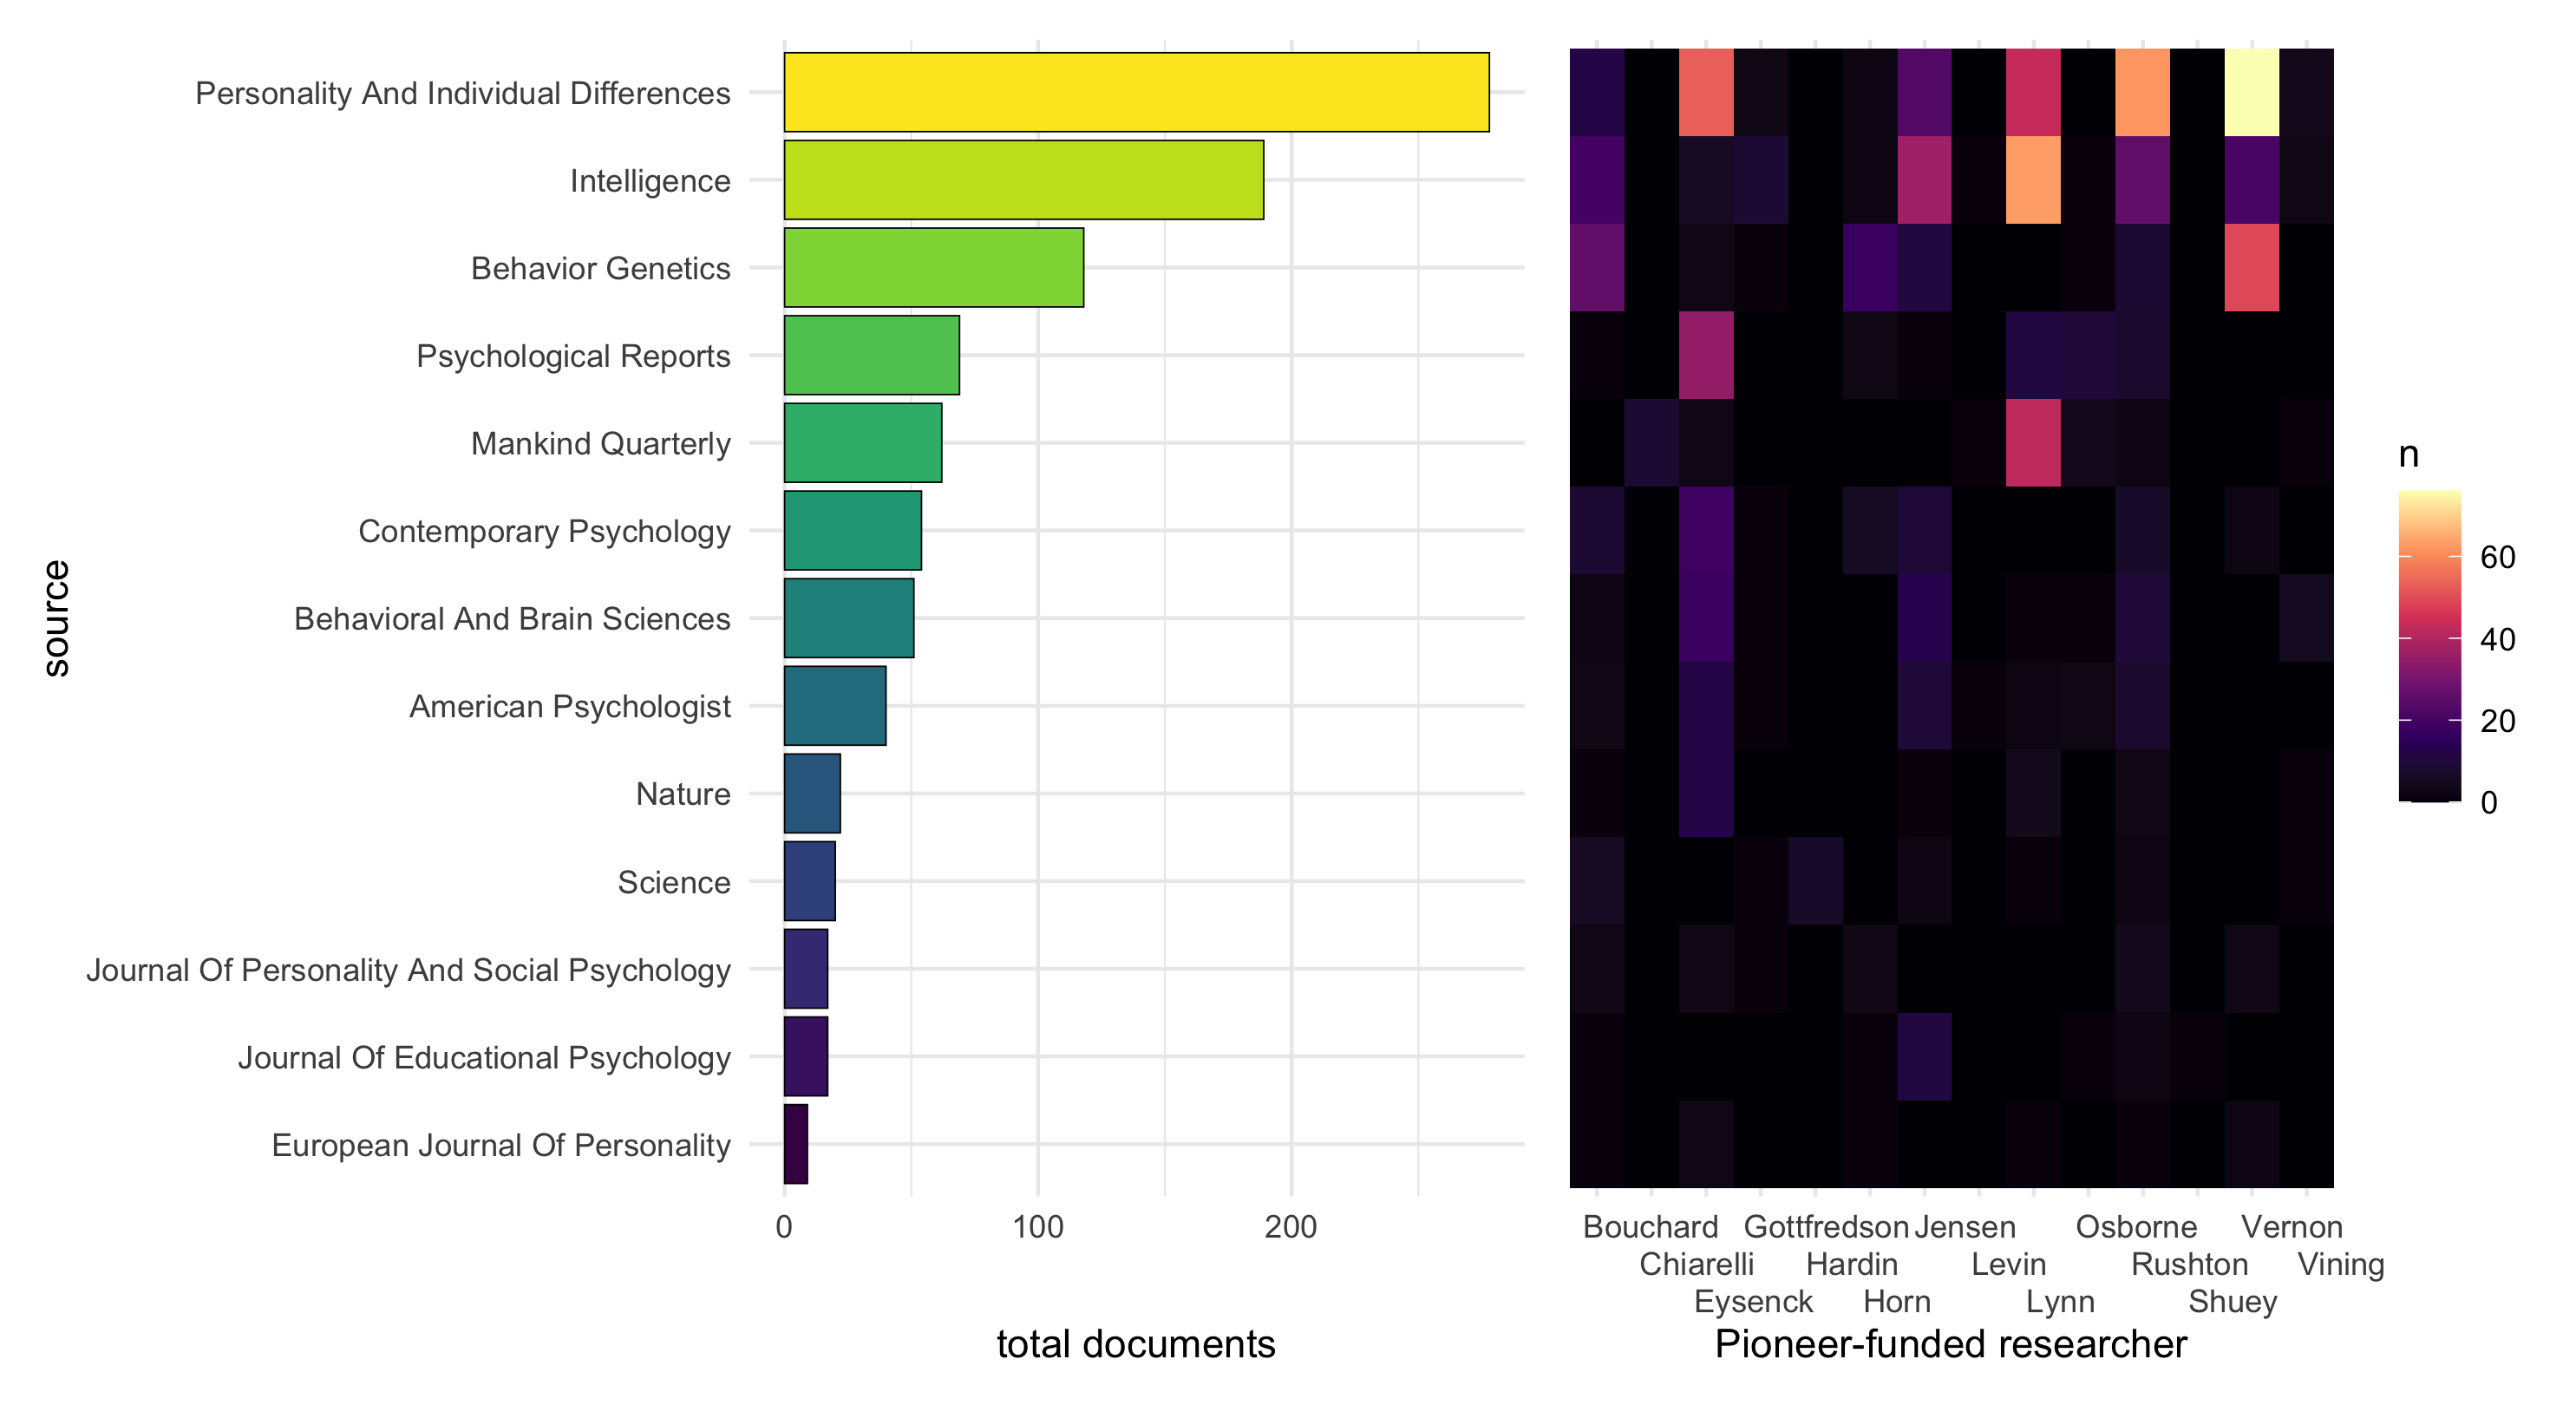
\includegraphics[width=4.76in,height=2.6in]{img/wos_results.png}
\caption{Journals publishing 6 or more Pioneer-funded researchers, Web of Science author search results \emph{{[}date coverage{]}} \label{fig:wos}}
\end{figure}

Figure \ref{fig:wos} shows that, while MQ is among the ``Pioneer-publishing'' journals, a number of mainstream journals are more prominent: \emph{Personality and Individual Differences} (PID), \emph{Intelligence} (I), \emph{Behavior Genetics} (BG), and \emph{Psychological Reports} (PR). In addition, only psychologist Richard Lynn appears to have published heavily in MQ. Lynn has been an assistant editor of MQ since 1979 \emph{{[}check this: \url{https://rationalwiki.org/wiki/Mankind_Quarterly}{]}} and president of PF since the death of psychologist J. Phillippe Rushton in 2012 \emph{{[}cite{]}}. By contrast, a number of Pioneer-funded researchers have published in PID, I, and to a lesser degree BG: Bouchard, Eysenck, Jensen, Rushton, Vernon, and also Lynn.

\emph{Personality and Individual Differences} (PID) was founded in 1980, with Eysenck as editor-in-chief and an editorial board including Jensen and Lynn. In the inaugural editorial, Eysenck identified ``studies of the genetic determinants of individual differences in the areas of personality and intelligence'' as one of the journal's eight major areas of interest. Eysenck remained editor-in-chief until his death in 1997. In 2005 the editorial board still included Jensen and Lynn. PID was first published by Pergamon Press, a mainstream academic press, and today is published by Elsevier. According to the Scimago Journal Rankings, based on Scopus citation data, in 2022 PID had an H-index of 193, \#29 in Psychology (Miscellaneous), and a 2-year citation index (impact factor) of 5.27, \#24 in Psychology (Miscellaneous).

\emph{Intelligence} (I) was founded in 1977, with psychologist Douglas Detterman as editor-in-chief from the founding until 2016. Lloyd Humphreys was on the editorial board starting from 1977; by 1990 he had been joined by Jensen and Philip Vernon. Richard Lynn joined the editorial board sometime between 1998 and 2002. (Archive copies of the I editorial board page are not available from the journal's website from 1999 through 2001.) I has been criticized for including Lynn and Gerhard Meisenberg on its editorial board until July-August 2018 \cite{SainiSuperiorReturnRace2019}. Meisenberg is also connected with the Pioneer Fund \emph{{[}director?{]}}, and was editor-in-chief of MQ in 2015-18 \emph{{[}check these{]}}. I is published by Elsevier. According to the Scimago Journal Rankings, based on Scopus citation data, in 2022 I had an H-index of 103, \#32 in Experimental and Cognitive Psychology, and a 2-year citation index (impact factor) of 3.05, \#31 in Experimental and Cognitive Psychology.

\hypertarget{topic-model-analysis}{%
\section*{Topic model analysis}\label{topic-model-analysis}}

The fact that Pioneer-funded researchers published heavily in two mainstream psychology journals does not tell us anything about the content of their publications or the findings of their research. We assembled a full-text corpus of articles published in MQ, PID, I, BG, PR, and Behavior and Brain Sciences (BBS) between 1960-2010 and used topic modeling to identify topics discussing race, intelligence, and both. \emph{{[}tables: Ns for each article, topic model parameters; figs: articles by pub over time, topic heatmaps, Silge plots, race-intelligence-both grids{]}}

\begin{figure}
\centering
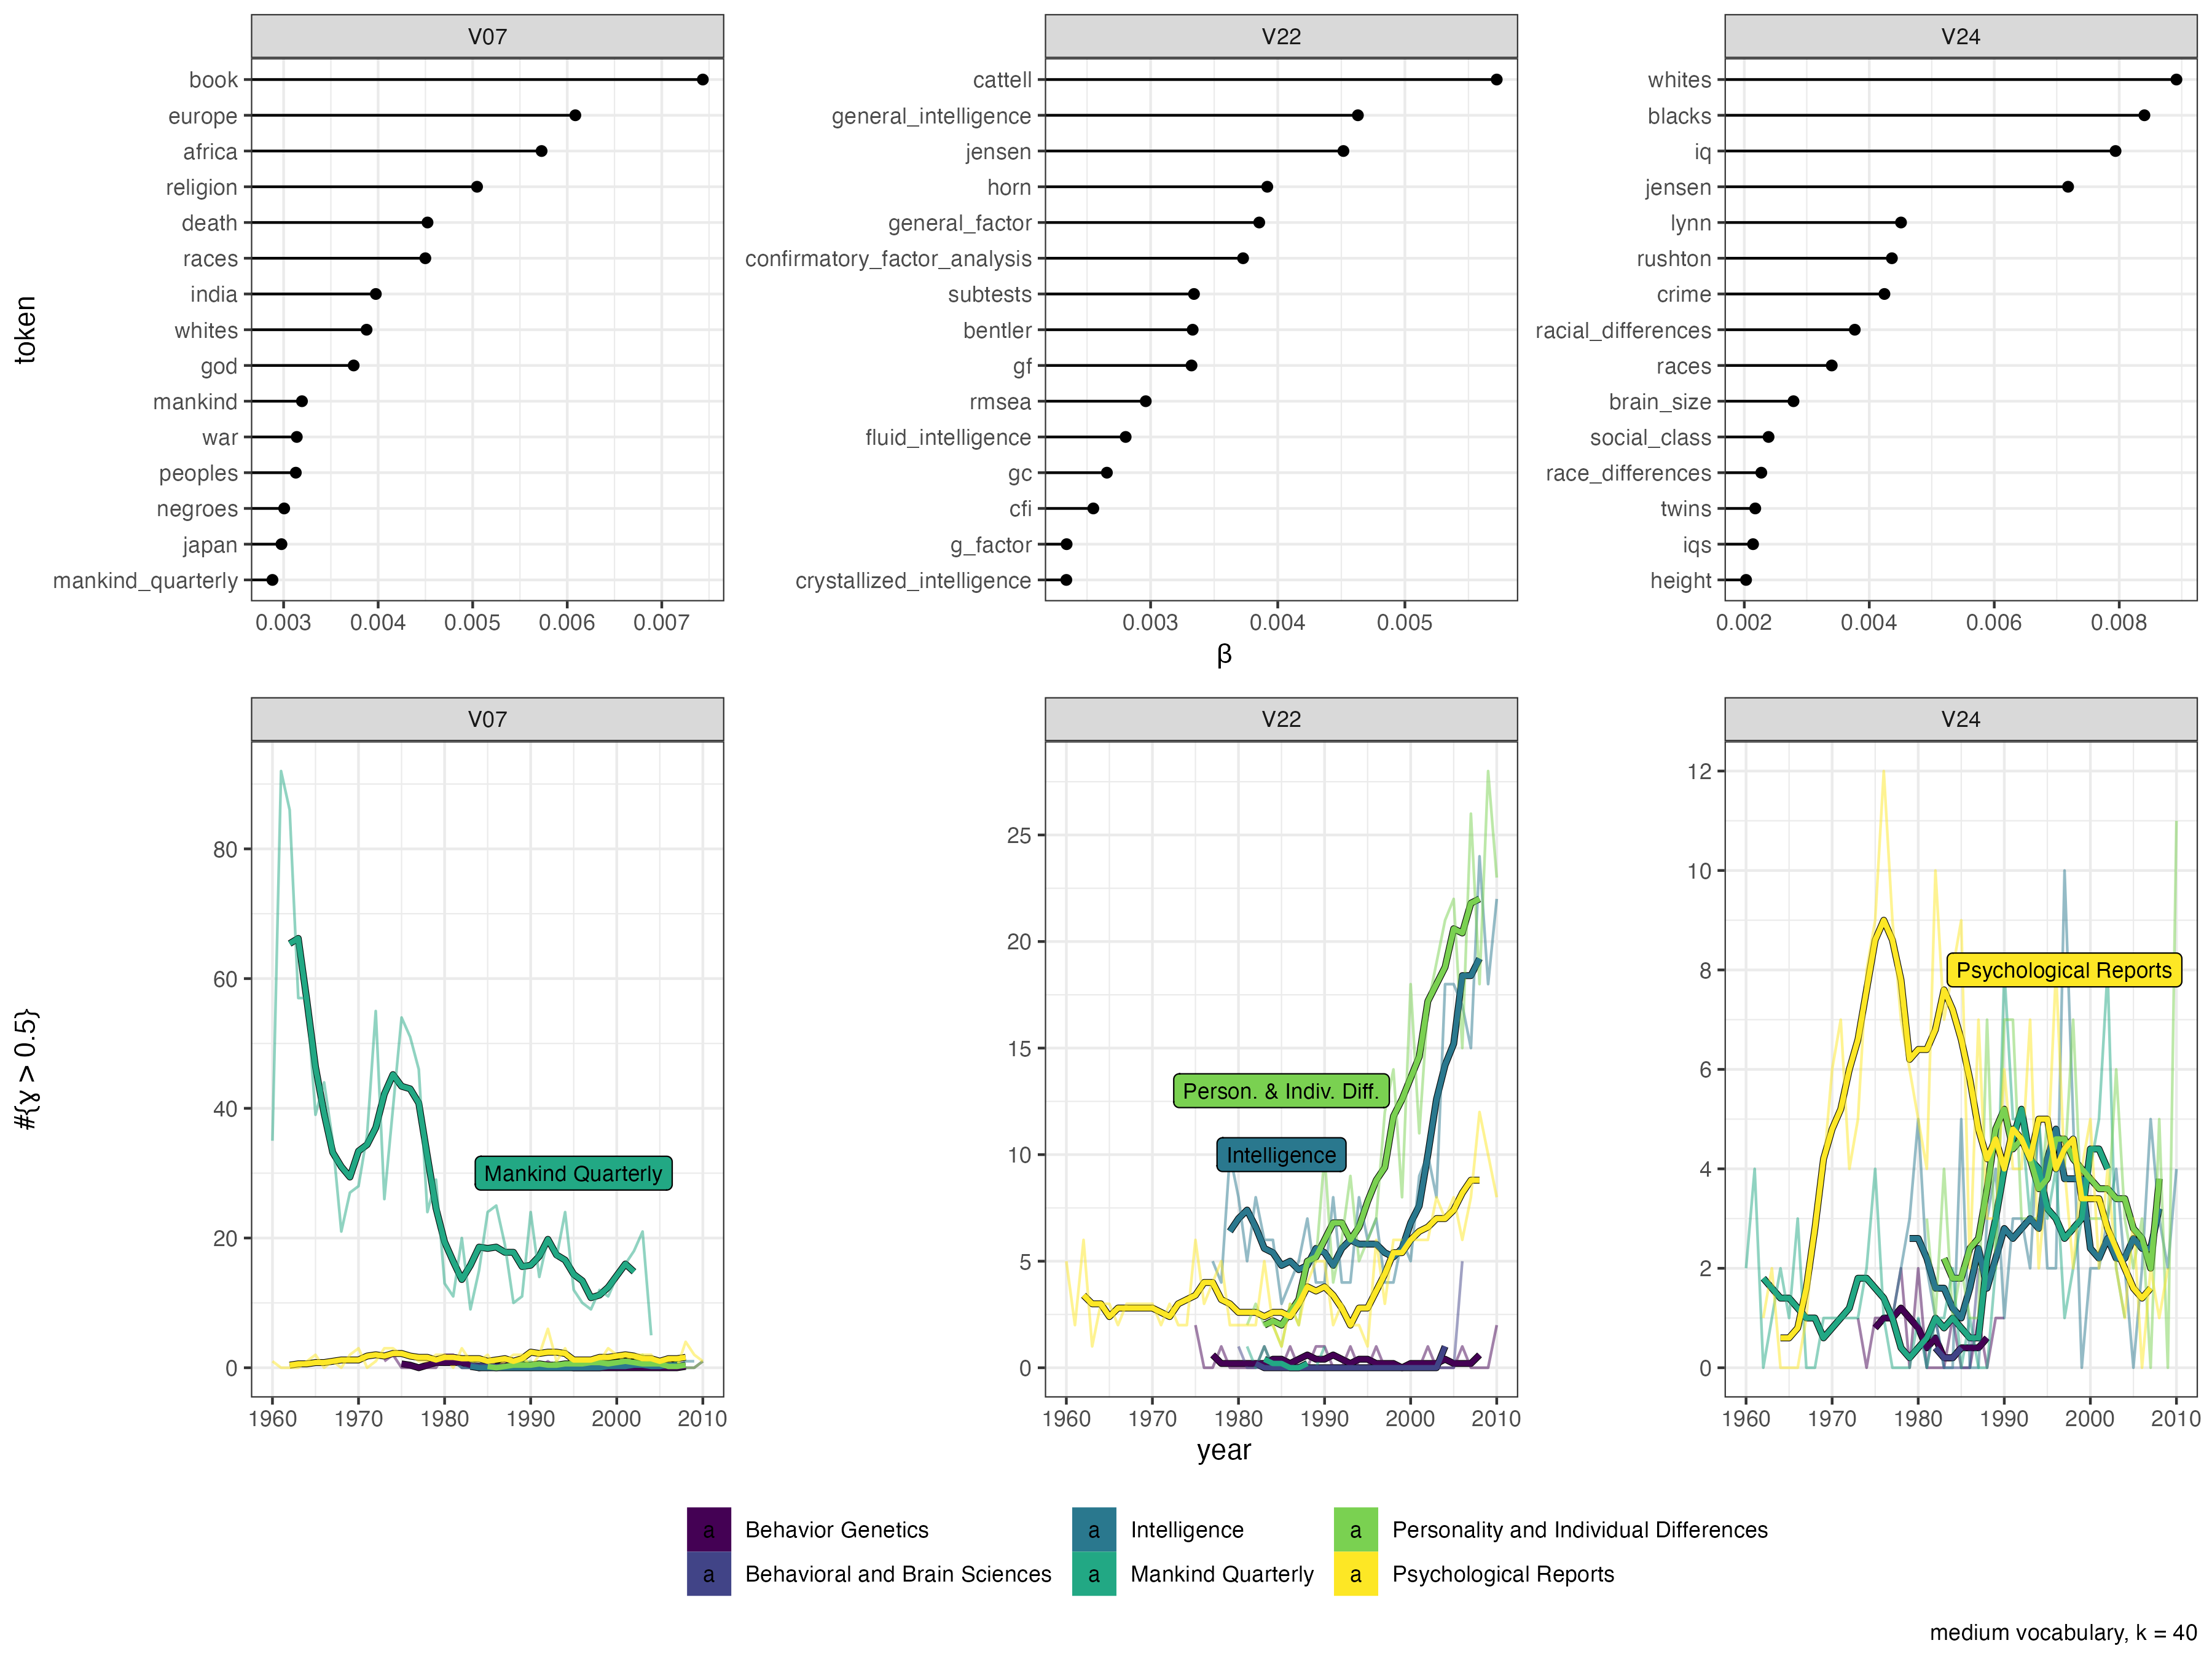
\includegraphics[width=4.76in,height=3.57in]{img/focal_topics.png}
\caption{Silge plots and smoothed time series for three focal topics. Top row: top 15 terms by \(\beta\) (term-topic distribution) for each topic. Bottom row: count of articles associated with each topic, by journal and year. Article counts use a threshold approach, with \(\gamma\) (topic-document distribution) greater than 0.5. Thin lines give annual values, thick lines give 5-year running averages. Because \emph{Behavior Genetics} and \emph{Behavioral and Brain Sciences} are not prominent in any panel, neither is given a direct label.}
\end{figure}

We focus here on three topics identified in one of the 24 fitted topic models \emph{{[}composite fig: topics over time + Silge plots{]}}. In this model, topic 07 is strongly associated with MQ: MQ published dozens of articles in this topic each year, and no other journal ever published more than a handful, with most other journals publishing none in a given year. The Silge plot contains racial terms (\texttt{races}, \texttt{whites}, \texttt{negroes} and potentially \texttt{europe}, \texttt{africa}, \texttt{india}, and \texttt{japan}) as well as \texttt{book}, likely reflecting the fact that MQ published a number of book reviews while the psychology journals did not.

Topic 22 is strongly associated with I and PID in the same way. The Silge plot does contain \texttt{jensen}, as well as a reference to Raymond Cattell, who played a major role in the development of factor analysis and intelligence testing also advocated eugenics, fascism, and Nazi race science\cite{MehlerBeyondismRaymondCattell1997}. However, the other authors named in this topic --- John Horn and Peter Bentler --- do not appear to have contributed to race science discourse. Instead this topic appears to identify ``mainstream'' (non-race science) intelligence research, specifically on factor analysis and the debate over whether intelligence in unidimensional or multidimensional. (Three other topics only associated with mainstream intelligence journals and terms were also identified by this topic model.) This topic indicates that the model is not simply lumping race science research together with other intelligence research.

The Silge plot for topic 24, by contrast, suggests a topic focused squarely on race and intelligence, with multiple racial terms (\texttt{whites}, \texttt{blacks}, \texttt{racial\_differences}, \texttt{races}, \texttt{race\_differences}) and the names of three prominent Pioneer-funded researchers, \texttt{jensen}, \texttt{lynn}, and \texttt{rushton}. To confirm this impression from the Silge plot, we independently coded the top 121 papers in this topic (those with \(gamma > 0.97\)) as contributing to race science discourse or not. 105 (87\%) were coded as race science discourse by both authors; 10 (8.3\%) were coded as not race science discourse by both; and discordant codes were given to the remaining 6 (5.0\%) (95\% agreement, Cohen's \(\kappa = 0.74\)).

In almost all years, most papers in topic 24 were published in mainstream journals rather than MQ. Jensen's ``How Much Can We Boost IQ and Scholastic Achievement?'' \cite{JensenHowMuchCan1969} was published in 1969 in Harvard Educational Review (not included in this study), and the time series indicates that, around this time, there was an increase in articles in topic 24 in both PS and MQ (the only two journals in our corpus that were active at the time). MQ shows another sharp increase in the late 1970s, around the time Lynn was brought on as assistant editor, \emph{{[}confirming the claim that Lynn shifted MQ's focus to intelligence research{]}}. PID published multiple papers in topic 24 almost immediately after it was founded, with I showing a more gradual increase between the mid-1970s and mid-1990s.

Notably, BG published very few articles in this topic. Outside of the field itself, behavior genetics is strongly associated with race science by both other academics and the general public. Panofsky \cite{PanofskyMisbehavingScienceControversy2014} argues that, prior to Jensen's 1969 paper, behavior genetics emphasized the study of non-human animals and intentionally avoided associations with eugenics and public controversy more generally. In response to Jensen, critics such as Lewontin offered broad critiques of behavior genetics as such, and behavior geneticists in turn adopted a radical conception of academic freedom (without any sense of responsibility for the social implications of academic research) and a siege or wartime mentality, as demonstrated by Sandra Scarr's 1986 presidential address to the Behavior Genetics Association (BGA) \cite{ScarrThreeCheersBehavior1987}. Scarr's address coincided with the period between 1970-1990 when BG published articles in topic 24 (including Scarr's address itself).

However, Glayde Whitney's 1995 BGA presidential address was published in MQ rather than BG. According to Whitney, BG's editor refused to publish the address and the BGA Executive Committee (except for Whitney himself) voted to ``issue an official statement of denouncement'' of the address; though we were unable to find any such a statement, and Panofsky reports that ``nothing official was done to Whitney.'' In his address, Whitney criticized ``the Marxist-Lysenkoist denial of genetics''; quoted Peter Brimelow --- a white nationalist and later founder of the racist and xenophobic website VDARE --- defining ``racist'' as ``anyone who is winning an argument with a liberal''; and proposed as a ``reasonable scientific hypothesis'' that differences in murder rates between countries and cities was caused by racial genetic differences in intelligence, empathy, aggression, and impulsivity.

The topic model analysis and the case of Whitney's address suggest that, by the 1990s, behavior genetics had at least somewhat distanced itself from race science, though perhaps without repudiating it. \emph{{[}\url{https://link.springer.com/search?use-oscar-shared-search=true\&sortBy=newestFirst\&dateTo=2010\&sortOrder=newestFirst\&facet-journal-id=10519\&content-type=Article\&query=race+intelligence\&date=custom\&dateFrom=\&date-facet-mode=between\&facet-start-year=1972\&previous-start-year=1972\&facet-end-year=2010\&previous-end-year=2023}{]}}

To check this interpretation, we ran an independent search for documents with the keywords ``race'' and ``intelligence'' published in BG from 1972 to 2020, using Springer's journal search website. This search returned 125 documents. 33 were presentation abstracts from meetings of the Behavior Genetics Association; we did not examine these further. 14 of the remaining documents were published since 2010 (after the scope of the primary study). Among these, one obituary and two papers celebrated the work of John Loehlin, a prominent race-and-intelligence researcher who had been Director of the American Eugenics Society from 1968-1972 \emph{{[}\url{http://link.springer.com/article/10.1007/s10519-020-10024-w}; \url{http://link.springer.com/article/10.1007/s10519-014-9687-1}; \url{http://link.springer.com/article/10.1007/s10519-014-9673-7}{]}}. Another was a retrospective of the work of Lindon Eaves, a geneticist who made at least one notable contribution to debates on the Scarr-Rowe hypothesis (interactions between heritability, race, and class). None of these 14 documents reported any studies of racial differences.

28 documents in this sample were published between 1990 and 2010. One was an obituary of Jerry Hirsch, a critic of hereditarianism in general and Jensen in particular \emph{{[}\url{http://link.springer.com/article/10.1007/s10519-008-9231-2}{]}}, and another was an obituary of David Rowe \emph{{[}\url{http://link.springer.com/article/10.1023/A\%3A1026122928868}{]}}. Only 2 of these 28 documents reported race differences of any kind: one examining at interactions among race, sex, and heritability for adolescent BMI (Body Mass Index, used as a measure of overweight/obesity) \emph{{[}\url{http://link.springer.com/article/10.1023/A\%3A1021619329904}{]}}; and the other at interactions among race, family history of alcoholism, and visuospatial performance \emph{{[}\url{http://link.springer.com/article/10.1007/BF02197241}{]}}. Finally, Philip Vernon --- one of the Pioneer-funded scientists we identified earlier --- published a critical review of a book that attempted to address hereditarianism, the Flynn effect, race-and-intelligence research, and some related issues.

This supplemental review provides additional support for the interpretation that behavior genetics had distanced itself from race science by the 1990s. Notably, this review brought our attention to a disciplinary history of behavior genetics published in 2010 \cite{McGueEndBehavioralGenetics2010}, which acknowledges the historical association with eugenics but does not mention Jensen and other race science controversies since World War II. Instead postwar behavior genetics is portrayed as an endeavor to counterbalance the hegemony of the ``Blank Slate,'' the supposedly widespread view that genetic differences play no role in explaining individual differences \cite{BatesonCorpseWearisomeDebate2002}. And none of the three documents celebrating Loehlin noted his postwar involvement in the eugenics movement. None of the documents examined in this supplemental review explicitly repudiate race science. Behavior geneticists seem to typically adopt a posture of objectivity and technical rigor, downplaying the extent of the field's involvement in race science in the past.

\hypertarget{discussion}{%
\section*{Discussion}\label{discussion}}

Our findings indicate that \emph{Mankind Quarterly} (MQ) was less important as an echo chamber for late 20th century race science than mainstream psychology journals, especially \emph{Intelligence} (I) and \emph{Personality and Individual Differences} (PID). Indeed, MQ published a very different kind of race science from the race-and-intelligence research published in I and PID, even after \emph{{[}Lynn joined the MQ editorial board{]}}.

We stress that we are not identifying any particular scientist as a racist based on the topic model results. Scientific research can be utilized to promote scientific racism --- and thus count as race science --- independently of the views and attitudes of the scientist who conducted that research.\cite{TaberyWhyStudyingGenetics2015, CarlsonQuantifyingContextualizingImpact2020, HennWhyDNANo2021} But this does not mean that scientists are not responsible for the downstream social effects of their
research, even when these effects involve deliberate misinterpretation.\emph{{[}Douglas, Kitcher, Kourany, Havstad; Block and Dworkin?{]}} Like other citizens, scientists are responsible for mitigating the reasonably foreseen harms that result from their actions. And we now have decades of empirical evidence that research on the genetics of intelligence --- even research that does not itself touch on race --- can and will be used to promote scientific racism.\cite{MeyerWrestlingSocialBehavioral2023}

\emph{{[}engagement dilemma: technical critiques can legitimize{]}}

\emph{{[}limitation: colorblind racism (Bonilla-Silva; WinstonWhyMainstreamResearch2020) creates coding ambiguities{]}}

\emph{{[}limitation: false negatives (race science papers that don't appear in V24) are possible if, eg, they use many terms related to twin studies of heritability and thereby appear in V03{]}}

\emph{{[}replace w/: WinstonWhyMainstreamResearch2020: race science as a community project of psychology(?). radical academic freedom is a tool used to defend race science PigliucciWhatAreWe2013, RosemanTroublesomeReflectionRacism2014, LarsenMoreProvocativeLess2020. an important part of how these mainstream journals function as race science echo chambers.{]}}

Proponents of a strong conception of academic freedom often point to chapter 2 of philosopher John Stuart Mill's \emph{On Liberty} \cite{MillLiberty1862}, ``Of the Liberty of Thought and Discussion.'' However, in chapter 1 of the same book, Mill states the Harm Principle as the overall thesis of his book: ``The only end for which people are entitled, individually or collectively, to interfere with the liberty of action of any of their number is self-protection. The only purpose for which power can be rightfully exercised over any member of a civilized community, against his will, is to prevent harm to others.'' Even for Mill, free speech and free inquiry are appropriately restrained when the ideas in question will harm others.

More recently, philosopher Shannon Dea \cite{DeaEvolvingSocialPurpose2021} has argued that academic freedom is importantly distinct from freedom of speech. Whereas freedom of speech is universal, enjoyed by all residents of countries where speech is legally protected, academic freedom is more exclusive, enjoyed only by college and university faculty. (Though, as Dea points out, non-tenure-track faculty often do not have effective protections for academic freedom.) Freedom of speech primarily serves to protect the interests of the individual speaker: that you will not be punished by the state for stating unpopular opinions. But academic freedom is ``other-directed,'' primarily serving to benefit the common good of society as a whole by enabling the pursuit of truth.

Advocates of research on genetics and intelligence --- both anti-racist liberals and race scientists --- claim this work will lead to social benefits. This reflects a recognition that the purpose of academic freedom is to promote the common good, rather than merely satisfy an individual's curiosity. But the promised benefits are either vague or do not actually require understanding the genetics of intelligence.\cite{KaplanGaltonQuincunxProbabilistic2021, CoopLotteryLuckLegacy2022}

Using agent-based models, Weatherall et al.\cite{WeatherallHowBeatScience2018} show that a strategy of ``selective sharing'' --- promoting favorable results from independent research --- can be effective at misleading a target audience.

\emph{{[}for discussion: the possibility for white supremacist appropriation, ie, race science done by scientists who are not themselves scientific racists: CarlsonQuantifyingContextualizingImpact2020; probably some reviews of Paige Harden; O'Connor and Weatherall{]}}

\emph{{[}what can science do? Posselt, /Equity in Science/{]}}

\emph{{[}max \textasciitilde50 refs{]}}
\bibliography{references.bib}
\bibliographystyle{Science}

% Following is a new environment, {scilastnote}, that's defined in the
% preamble and that allows authors to add a reference at the end of the
% list that's not signaled in the text; such references are used in
% *Science* for acknowledgments of funding, help, etc.

\begin{scilastnote}
\item \emph{{[}strutured{]}} Thanks to Emily Merchant and John Jackson for some initial discussions that helped clarify the scope of the project and identify some key resources related to the Pioneer Fund and \emph{Mankind Quarterly}. Thanks to Anthony Sainez for help retrieving the \emph{Mankind Quarterly} articles. Thanks to Derek Devnich and James Dooley for their work attempting to secure the APA-published articles. EL's work on this project was supported by UC Merced. DH's work on this project was not supported by any specific funding.
\end{scilastnote}


\renewcommand{\thetable}{\arabic{table}}
\renewcommand{\thefigure}{\arabic{figure}}
\setcounter{table}{0}
\setcounter{figure}{0}

%%%begfigs---

%%%endfigs---

%%%begtabs---

%%%endtabs---

% Needs a bit of work on the \ref{} TODO  before uncommenting
%\renewcommand{\thetable}{A\arabic{table}}
%\renewcommand{\thefigure}{A\arabic{figure}}
%\setcounter{table}{0}
%\setcounter{figure}{0}

%%%begappxfigs---

%%%endappxfigs---

%%%begappxtabs---

%%%endappxtabs---

\end{document}
